\documentclass[12pt,a4paper]{report}

\usepackage[utf8]{inputenc}
\usepackage[T1]{fontenc}
\usepackage[french]{babel}
\usepackage[a4paper,margin=2.5cm]{geometry}
\usepackage{graphicx}
\usepackage{float}
\usepackage{booktabs}
\usepackage{array}
\usepackage{tabularx}
\usepackage{xcolor}
\usepackage{hyperref}
\usepackage{enumitem}
\usepackage{tikz}
\usetikzlibrary{arrows.meta,positioning,shapes.geometric}
\usepackage{setspace}
\usepackage{parskip}

\definecolor{primary}{RGB}{30, 60, 114}
\definecolor{accent}{RGB}{0, 150, 199}
\definecolor{successgreen}{RGB}{39, 174, 96}
\definecolor{warnred}{RGB}{192, 57, 43}
\definecolor{warnyellow}{RGB}{241, 196, 15}

\hypersetup{
  colorlinks=true,
  linkcolor=primary,
  urlcolor=accent,
  citecolor=primary,
  pdftitle={Implémentation du RAG Agentique - Rapport d'Avancement},
  pdfauthor={Brahim Bazi et Youcef El Omari}
}

\setcounter{tocdepth}{2}
\onehalfspacing

\begin{document}

\begin{titlepage}
  \centering
  \begin{minipage}{0.18\textwidth}
    \centering
    
\includegraphics[width=\textwidth]{uizpic.png}
  \end{minipage}
  \hfill
  \begin{minipage}{0.18\textwidth}
    \centering
    
\includegraphics[width=\textwidth]{3D-SMART-FACTORY.png}
  \end{minipage}

  \vspace{2cm}

  {\Large État d'avancement hebdomadaire\par}
  \vspace{0.7cm}
  {\Huge\bfseries Implémentation du RAG Agentique\par}
  \vspace{0.4cm}
  {\LARGE Rapport d'Avancement\par}
  \vspace{1.2cm}

  {\large Difficultés, architecture et feuille de route\par}
  \vfill

  \begin{tabular}{rl}
    \textbf{Auteurs :} & Brahim BAZI \\
                       & Youcef EL OMARI \\
    \textbf{Encadrant :} & M. Thierry BERTIN \\
    \textbf{Date :} & 15 mars 2026 \\
  \end{tabular}

  \vfill

  {\large Projet RAG multi-agents pour la gestion de connaissances\par}
\end{titlepage}

\tableofcontents
\clearpage

\chapter*{Résumé}
\addcontentsline{toc}{chapter}{Résumé}

Ce rapport présente l'état d'avancement de l'implémentation d'un système de \textit{Retrieval-Augmented Generation} (RAG) agentique inspiré d'une architecture multi-agents. Le travail réalisé cette semaine s'est concentré sur trois axes principaux : l'analyse des performances de trois variantes d'implémentation, la consolidation de l'architecture logicielle à cinq agents, et l'identification des optimisations prioritaires à développer pour les prochaines itérations.

Les benchmarks montrent que l'approche hybride, combinant Python pour l'orchestration et Rust pour les composants critiques, offre les meilleurs résultats en latence et en stabilité. En parallèle, l'architecture multi-agents est désormais fonctionnelle, avec un mécanisme d'évaluation automatisée de la réponse et une boucle de raffinement contrôlée. Enfin, plusieurs pistes d'amélioration ont été identifiées, notamment l'introduction d'un retrieval hybride, un routage conditionnel des agents et la migration vers un LLM local.

\chapter{Introduction et contexte}

L'objectif de ce projet est de concevoir un système RAG agentique capable de produire des réponses fondées sur un corpus documentaire tout en intégrant une logique de contrôle qualité. Contrairement à un pipeline RAG classique, qui se limite généralement à une étape de récupération suivie d'une génération, l'approche choisie ici repose sur plusieurs agents spécialisés qui coopèrent autour d'un état partagé.

Le système s'inspire du travail de Amaram et al. sur les assistants IA pour la gestion des connaissances et la formation professionnelle. L'ambition n'est pas de reproduire à l'identique leur environnement expérimental, mais d'adapter les principes de leur architecture à notre propre pile technique et à nos contraintes de développement.

Cette semaine, l'effort principal a porté sur la validation technique de l'architecture et sur la mesure rigoureuse de ses performances. Les résultats présentés dans ce document permettent d'établir une base solide pour les prochaines itérations du projet.

\chapter{Résultats des tests de latence}

\section{Protocole expérimental}

Les tests de performance ont été réalisés sur un pipeline RAG simple afin de comparer le coût d'exécution de trois variantes d'implémentation :

\begin{itemize}[leftmargin=1.2cm]
  \item \textbf{100\% Python} : implémentation classique de bout en bout.
  \item \textbf{100\% Rust} : implémentation native optimisée.
  \item \textbf{Hybride} : orchestration en Python avec modules critiques en Rust.
\end{itemize}

Pour garantir une comparaison cohérente, le protocole suivant a été appliqué :

\begin{itemize}[leftmargin=1.2cm]
  \item 100 exécutions successives du pipeline ;
  \item une même requête d'entrée ;
  \item un même corpus documentaire ;
  \item une mesure systématique des latences sur les étapes clés.
\end{itemize}

L'objectif de cette campagne de tests est double : identifier le principal goulot d'étranglement du système et déterminer quelle architecture offre le meilleur compromis entre performance, stabilité et facilité d'évolution.

\section{Temps moyen de génération des embeddings}

La première mesure porte sur la génération des embeddings, qui constitue une étape critique dans la plupart des systèmes RAG.

\begin{figure}[H]
  \centering
  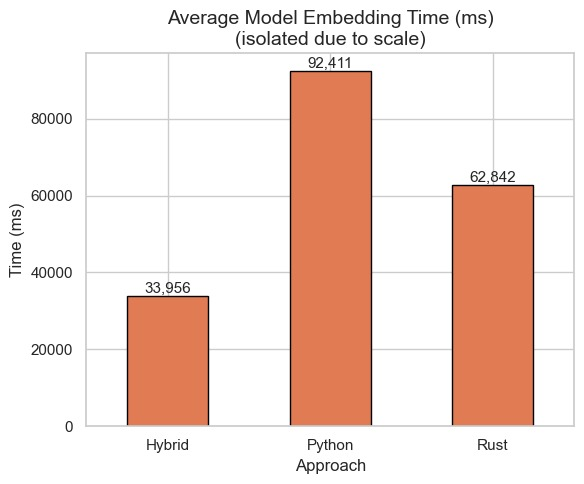
\includegraphics[width=0.88\textwidth]{average_model_embeddings_time_ms.jpg}
  \caption{Temps moyen de génération des embeddings en millisecondes.}
\end{figure}

Les résultats montrent que cette étape représente le principal goulot d'étranglement du pipeline. L'approche hybride obtient la meilleure latence moyenne, ce qui confirme l'intérêt d'externaliser les composants intensifs vers Rust tout en conservant Python pour l'orchestration globale. L'implémentation Rust arrive en deuxième position et demeure très performante. L'approche Python pure, en revanche, reste la plus lente.

Cette hiérarchie confirme qu'une optimisation ciblée des composants coûteux est plus rentable qu'une réécriture complète du pipeline lorsqu'on cherche à améliorer rapidement les performances sans sacrifier la flexibilité.

\section{Temps d'exécution du pipeline hors embeddings}

Afin d'isoler le coût structurel du pipeline, une seconde mesure a été réalisée en excluant le temps de génération des embeddings.

\begin{figure}[H]
  \centering
  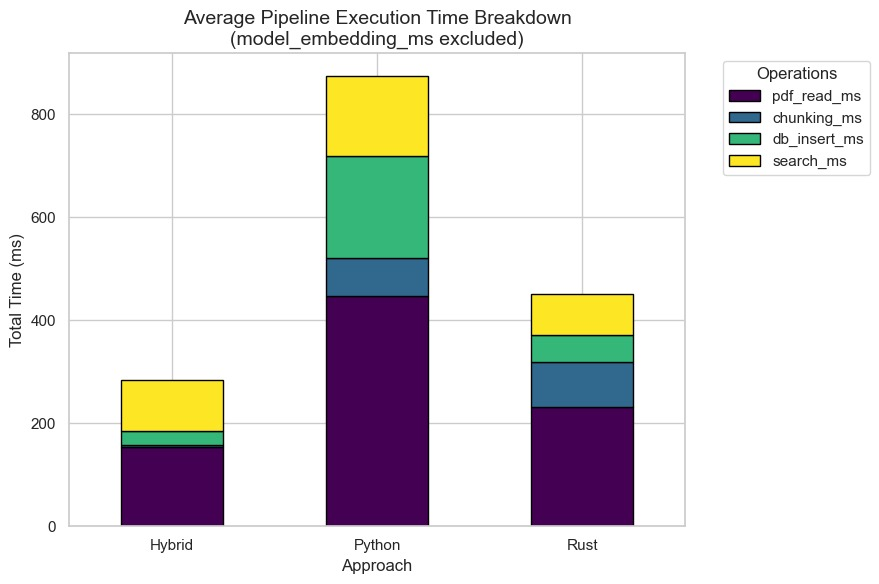
\includegraphics[width=0.88\textwidth]{average_pipeline_execution_time_model_embeddings_ms excluded.jpg}
  \caption{Temps d'exécution moyen du pipeline hors génération des embeddings.}
\end{figure}

Cette mesure permet d'observer la latence liée au traitement interne du pipeline RAG, indépendamment du coût des modèles d'embedding. Ici encore, l'approche hybride se révèle la plus rapide. Cela suggère que les gains observés ne proviennent pas uniquement de l'étape d'embedding, mais aussi d'une meilleure efficacité sur l'ensemble de la chaîne de traitement.

L'implémentation Rust se positionne de nouveau comme une alternative très performante, tandis que Python reste en retrait. La conclusion opérationnelle est claire : pour un système destiné à évoluer vers la production, l'architecture hybride constitue aujourd'hui le meilleur compromis.

\section{Analyse des tendances sur 100 exécutions}

Au-delà de la moyenne, il est essentiel d'évaluer la stabilité temporelle des différentes approches. La figure suivante illustre l'évolution des performances sur l'ensemble des 100 runs.

\begin{figure}[H]
  \centering
  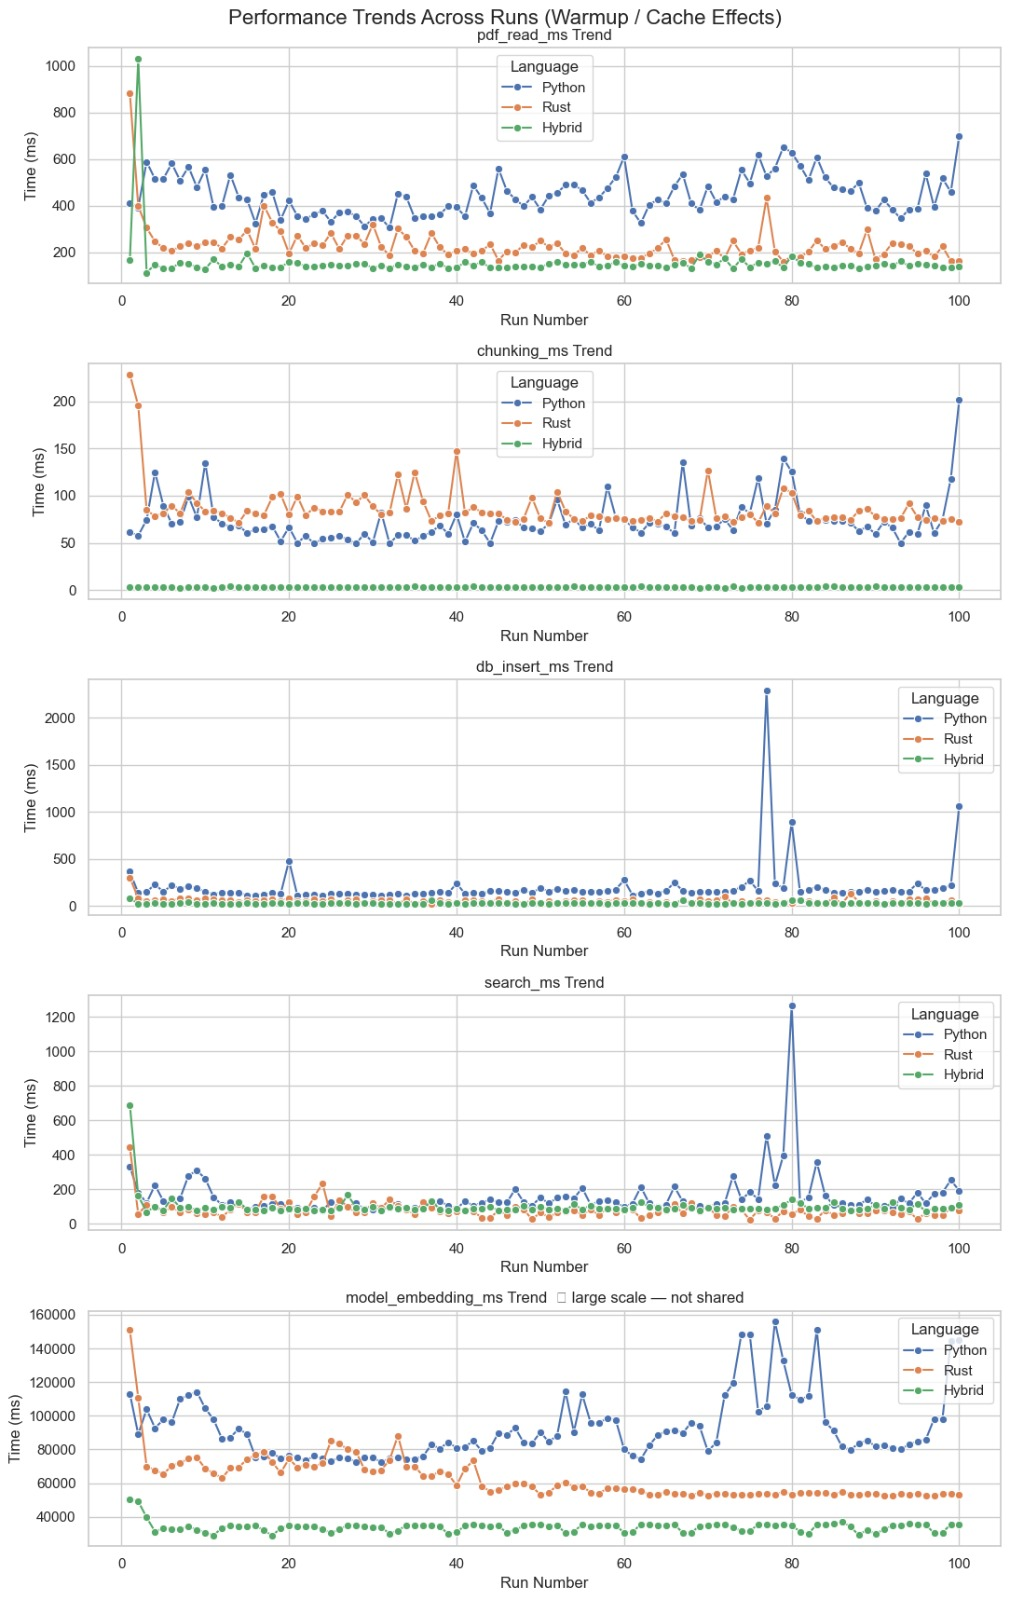
\includegraphics[width=0.72\textwidth]{performance_trends_accross_runs.jpg}
  \caption{Tendances de performance sur 100 exécutions successives.}
\end{figure}

L'approche Python présente des pics de latence occasionnels, probablement liés au \textit{garbage collector}, aux allocations mémoire et à la variabilité d'exécution. À l'inverse, Rust et l'approche hybride produisent des courbes plus régulières et plus prévisibles.

Cette prévisibilité est particulièrement importante dans un contexte de production, où l'on cherche à maîtriser non seulement la latence moyenne, mais aussi la variance. Un système dont les temps de réponse sont stables est plus simple à superviser, à dimensionner et à intégrer dans une application réelle.

\section{Synthèse}

Le tableau suivant résume les conclusions qualitatives des benchmarks.

\begin{table}[H]
  \centering
  \renewcommand{\arraystretch}{1.25}
  \small
  \begin{tabularx}{\textwidth}{>{\bfseries}p{4.2cm} >{\centering\arraybackslash}X >{\centering\arraybackslash}X >{\centering\arraybackslash}X}
    \toprule
    Critère & Python & Rust & Hybride \\
    \midrule
    Latence des embeddings & Faible performance & Bonne performance & Meilleure performance \\
    Latence du pipeline & Faible performance & Bonne performance & Meilleure performance \\
    Stabilité inter-runs & Variable & Stable & Très stable \\
    Simplicité de développement & Élevée & Moyenne & Bonne \\
    \bottomrule
  \end{tabularx}
  \caption{Synthèse comparative des trois approches testées.}
\end{table}

En conclusion, l'approche hybride domine les trois benchmarks observés. L'implémentation Rust seule reste très solide, mais l'approche hybride bénéficie d'un meilleur équilibre entre performances et souplesse de développement. Python seul demeure intéressant pour le prototypage rapide, mais montre ses limites dès que la performance devient un critère central.

\chapter{Architecture multi-agents}

\section{Vue d'ensemble}

Le système cible repose sur cinq agents spécialisés, coordonnés par un agent proxy. Chaque agent intervient sur une responsabilité précise, ce qui améliore la modularité du pipeline et facilite l'introduction de stratégies de contrôle qualité.

\begin{figure}[H]
  \centering
  \resizebox{\textwidth}{!}{
  \begin{tikzpicture}[
    node distance=0.8cm and 0.7cm,
    agent/.style={
      rectangle,
      rounded corners=4pt,
      minimum width=2.5cm,
      minimum height=0.95cm,
      draw=primary,
      fill=primary!10,
      text=primary,
      align=center,
      font=\bfseries
    },
    flow/.style={-{Stealth[length=5pt]}, thick, color=accent},
    retry/.style={-{Stealth[length=5pt]}, thick, dashed, color=warnred},
    success/.style={-{Stealth[length=5pt]}, thick, color=successgreen}
  ]
    \node[agent] (proxy) {Agent Proxy\\Utilisateur};
    \node[agent, right=of proxy] (refiner) {Agent\\Raffineur};
    \node[agent, right=of refiner] (retriever) {Agent\\Retriever};
    \node[agent, right=of retriever] (generator) {Agent\\Générateur};
    \node[agent, right=of generator] (evaluator) {Agent\\Évaluateur};

    \draw[flow] (proxy) -- node[above] {\small requête} (refiner);
    \draw[flow] (refiner) -- node[above] {\small requête affinée} (retriever);
    \draw[flow] (retriever) -- node[above] {\small contexte} (generator);
    \draw[flow] (generator) -- node[above] {\small brouillon} (evaluator);

    \draw[retry] (evaluator.south) -- ++(0,-0.8) -| node[below,pos=0.2] {\small score faible $\Rightarrow$ réessai} (refiner.south);
    \draw[success] (evaluator.north) -- ++(0,0.8) node[right] {\small réponse finale};
  \end{tikzpicture}}
  \caption{Architecture du pipeline RAG multi-agents.}
\end{figure}

Cette organisation permet de séparer la récupération d'information, la génération, l'évaluation et le raffinement. Le bénéfice principal est la possibilité de corriger dynamiquement une réponse insuffisante au lieu de dépendre d'un unique passage linéaire.

\section{Rôle des agents}

\begin{itemize}[leftmargin=1.2cm]
  \item \textbf{Agent Proxy Utilisateur} : point d'entrée du système, il orchestre le pipeline global et gère la boucle de réessai.
  \item \textbf{Agent Raffineur} : reformule la requête initiale pour améliorer la qualité de la récupération.
  \item \textbf{Agent Retriever} : recherche les passages les plus pertinents dans la base vectorielle à partir de la requête.
  \item \textbf{Agent Générateur} : produit une réponse fondée sur le contexte récupéré.
  \item \textbf{Agent Évaluateur} : note la réponse et décide si une nouvelle itération est nécessaire.
\end{itemize}

Le découpage en agents offre également une base saine pour l'expérimentation future. Il devient par exemple simple d'ajouter un reranker, un routeur ou un agent de décomposition de requêtes sans bouleverser le fonctionnement global.

\section{Communication entre agents via un \textit{State Dict}}

Le mécanisme de communication retenu repose sur un dictionnaire d'état partagé en Python. Chaque agent lit certaines clés et en enrichit d'autres, sans dépendre directement des implémentations des agents voisins. Le contrôle du flux reste ainsi centralisé dans l'orchestrateur.

\begin{table}[H]
  \centering
  \renewcommand{\arraystretch}{1.25}
  \begin{tabularx}{\textwidth}{>{\ttfamily}l X}
    \toprule
    Clé & Rôle \\
    \midrule
    query & requête originale soumise par l'utilisateur \\
    refined\_query & version reformulée de la requête pour améliorer la récupération \\
    chunks & contexte documentaire récupéré par le retriever \\
    answer & réponse générée par l'agent générateur \\
    score & score attribué par l'évaluateur \\
    attempts & nombre d'itérations déjà effectuées \\
    should\_retry & booléen indiquant si une nouvelle tentative est nécessaire \\
    \bottomrule
  \end{tabularx}
  \caption{Structure logique du dictionnaire d'état partagé.}
\end{table}

Ce choix présente plusieurs avantages : il découple les agents, facilite le débogage, améliore la traçabilité de l'exécution et évite l'introduction prématurée d'un framework plus lourd. Il s'agit d'une approche pragmatique, adaptée à la phase actuelle du projet.

\section{Évaluation automatique de la réponse}

L'agent évaluateur repose sur un schéma de type \textit{LLM-as-a-Judge}. Son rôle est d'attribuer une note à la réponse générée en fonction de deux critères principaux :

\begin{itemize}[leftmargin=1.2cm]
  \item \textbf{Faithfulness} : la réponse reste-t-elle fidèle au contexte récupéré ?
  \item \textbf{Relevance} : la réponse répond-elle réellement à la question posée ?
\end{itemize}

Le LLM produit un court raisonnement, suivi d'un score sous une forme structurée telle que \texttt{SCORE: 0.95}. Ce score est ensuite extrait automatiquement via une expression régulière, puis comparé à un seuil prédéfini. Si le score est inférieur au seuil et que le nombre maximal de tentatives n'est pas atteint, la variable \texttt{should\_retry} passe à vrai et le pipeline relance un cycle de raffinement.

Ce mécanisme introduit une capacité d'auto-correction dans le système. Il s'agit d'une évolution importante par rapport à un pipeline RAG classique, qui génère une réponse sans mécanisme natif de contrôle qualité.

\section{Optimisations actuelles}

\subsection{Préfixe BGE pour la requête}

Le retriever exploite un modèle BGE pour les embeddings. Ce type de modèle recommande l'ajout d'un préfixe explicite à la requête, du type :

\begin{quote}
Represent this sentence for searching relevant passages: \{query\}
\end{quote}

Ce préfixe est appliqué uniquement à la requête utilisateur, et non aux morceaux de documents indexés. Cette adaptation améliore la qualité de la recherche vectorielle, ce qui a un impact direct sur la pertinence des réponses générées.

\subsection{Cache par hash SHA-256}

Le pipeline intègre également un mécanisme de cache basé sur un hash SHA-256 des fichiers PDF et des paramètres de \textit{chunking}. Tant que les documents sources ne changent pas, le système évite de recalculer les embeddings. Cette optimisation réduit très fortement le temps de réindexation et limite les coûts d'appel aux modèles, qu'ils soient distants ou locaux.

\chapter{Stack technique et état d'avancement}

\section{Pile technique actuelle}

L'implémentation actuelle s'appuie sur une stack mixte pensée pour conjuguer rapidité de développement et performance :

\begin{itemize}[leftmargin=1.2cm]
  \item \textbf{Langage principal} : Python, complété par des modules Rust via PyO3.
  \item \textbf{LLM} : API OpenRouter pour l'appel à des modèles distants.
  \item \textbf{Embeddings} : \texttt{fastembed} avec ONNX Runtime et le modèle BGE-Small-EN-v1.5, utilisé depuis Rust.
  \item \textbf{Base vectorielle} : LanceDB via ses bindings Rust.
  \item \textbf{Ingestion PDF} : \texttt{pdf-oxide} combiné à Rayon pour le traitement parallèle.
  \item \textbf{Exposition applicative} : FastAPI pour la couche REST.
\end{itemize}

Cette pile reflète une stratégie claire : utiliser Python pour la coordination, les API et la logique d'orchestration, tout en déportant les traitements critiques vers des composants natifs plus efficaces.

\section{Fonctionnalités déjà opérationnelles}

À ce stade, plusieurs briques majeures sont déjà disponibles :

\begin{itemize}[leftmargin=1.2cm]
  \item pipeline complet à cinq agents ;
  \item boucle de raffinement itérative avec nombre maximal de tentatives ;
  \item cache SHA-256 pour éviter les réindexations inutiles ;
  \item évaluateur de type \textit{LLM-as-a-Judge} ;
  \item préfixe BGE pour améliorer le retrieval ;
  \item benchmark des trois variantes Python, Rust et hybride ;
  \item déploiement Docker fonctionnel.
\end{itemize}

Ces avancées montrent que le projet a dépassé le stade du prototype conceptuel. L'effort peut désormais se concentrer sur l'amélioration de la qualité de récupération, la réduction du coût des appels LLM et l'évaluation reproductible.

\section{État des tâches}

\begin{table}[H]
  \centering
  \renewcommand{\arraystretch}{1.25}
  \begin{tabular}{>{\bfseries}c p{9cm} l}
    \toprule
    \# & Tâche & Statut \\
    \midrule
    1 & Cache SHA-256 des embeddings & Fait \\
    2 & LLM-as-a-Judge pour l'évaluation & Fait \\
    3 & Préfixe BGE pour la récupération & Fait \\
    4 & Implémentation du retrieval hybride (BM25 + dense) & En cours \\
    5 & Routage conditionnel des agents & En cours \\
    6 & Installation et configuration d'Ollama en local & À faire \\
    7 & Mise en place de RAGAS / DeepEval & À faire \\
    \bottomrule
  \end{tabular}
  \caption{État d'avancement des travaux techniques.}
\end{table}

\chapter{Démonstration}

Une démonstration vidéo du système a été préparée afin d'illustrer le comportement global du pipeline. Elle permet d'observer l'enchaînement des étapes de récupération, de génération et d'évaluation dans un scénario réel.

Le lien de démonstration est accessible ici :

\begin{center}
  \url{https://drive.google.com/file/d/1epr5hFfWa-HFFunyXydkKVBxAFvzkRtH/view}
\end{center}

Cette démonstration complète les résultats expérimentaux en donnant une vue qualitative de l'expérience utilisateur et du comportement du système au fil de l'exécution.

\chapter{Prochaines étapes}

\section{Tâches prioritaires}

Trois axes de travail apparaissent comme prioritaires pour la suite du projet :

\begin{enumerate}[leftmargin=1.2cm]
  \item \textbf{Retrieval hybride} : combiner BM25 et dense retrieval avec une stratégie de fusion de rangs telle que \textit{Reciprocal Rank Fusion}. L'objectif est d'améliorer le rappel sur les requêtes complexes ou partiellement formulées.
  \item \textbf{Routage conditionnel} : éviter d'appeler systématiquement tous les agents lorsque la qualité de récupération est déjà suffisante. Une telle optimisation permettrait de réduire le nombre d'appels LLM et donc la latence ainsi que les coûts.
  \item \textbf{Migration d'OpenRouter vers Ollama} : exécuter un LLM local afin de réduire la dépendance réseau, de limiter les coûts d'exploitation et d'améliorer la maîtrise de l'environnement d'inférence.
\end{enumerate}

\section{Objectifs secondaires}

En complément des priorités immédiates, plusieurs améliorations importantes ont été identifiées :

\begin{itemize}[leftmargin=1.2cm]
  \item ajout d'un reranker \textit{cross-encoder} pour améliorer la précision finale ;
  \item décomposition des requêtes complexes en sous-requêtes spécialisées ;
  \item intégration de RAGAS ou DeepEval pour obtenir des métriques reproductibles ;
  \item enrichissement du corpus documentaire afin de tester le système sur des données plus représentatives.
\end{itemize}

\section{Plan d'action}

\begin{table}[H]
  \centering
  \renewcommand{\arraystretch}{1.25}
  \begin{tabular}{>{\bfseries}c p{9cm} l}
    \toprule
    \# & Action & Horizon \\
    \midrule
    1 & Finaliser le retrieval hybride BM25 + dense & Court terme \\
    2 & Implémenter le routage conditionnel des agents & Court terme \\
    3 & Installer et configurer Ollama en local & Court terme \\
    4 & Intégrer un reranker et tester son impact & Moyen terme \\
    5 & Mettre en place une évaluation automatisée avec RAGAS / DeepEval & Moyen terme \\
    6 & Étendre et diversifier le corpus de test & Moyen terme \\
    \bottomrule
  \end{tabular}
  \caption{Plan d'action synthétique pour les prochaines itérations.}
\end{table}

\chapter{Conclusion}

Le projet a franchi une étape importante. Les résultats de performance montrent qu'une architecture hybride Python/Rust est aujourd'hui la plus prometteuse pour porter un RAG agentique performant. En parallèle, l'architecture multi-agents à cinq rôles est désormais mise en place avec une logique d'évaluation et de réessai qui rapproche le système d'un fonctionnement autonome.

Les prochaines semaines devront maintenant transformer cette base fonctionnelle en système plus robuste et plus efficace. L'amélioration du retrieval, la réduction du coût des appels LLM et l'introduction de métriques d'évaluation formelles constitueront les leviers principaux pour passer d'un prototype avancé à une plateforme expérimentale crédible.

\appendix
\chapter{Référence}

\begin{thebibliography}{1}

\bibitem{amaram2026}
Amaram et al.,
\textit{Developing an AI Assistant for Knowledge Management and Workforce Training in State DOTs},
arXiv:2603.03302v1, février 2026.

\end{thebibliography}

\end{document}
